\documentclass{article}

\usepackage{GOST}
\usepackage[T1, T2A]{fontenc}
\usepackage[utf8]{inputenc}
\usepackage[russian]{babel}
\usepackage{titlesec}
\usepackage{cmap}
\usepackage{amssymb}
\usepackage{amsmath}
\usepackage{hyperref}
\usepackage{tabularx}
\usepackage{listings}
\usepackage{float}
% Для листинга кода:
\lstset{ 
	language=C,                 % выбор языка для подсветки (здесь это С)
	basicstyle=\small\sffamily, % размер и начертание шрифта для подсветки кода
	numbers=left,               % где поставить нумерацию строк (слева\справа)
	numberstyle=\tiny,           % размер шрифта для номеров строк
	stepnumber=1,                   % размер шага между двумя номерами строк
	numbersep=5pt,                % как далеко отстоят номера строк от подсвечиваемого кода
	showspaces=false,            % показывать или нет пробелы специальными отступами
	showstringspaces=false,      % показывать или нет пробелы в строках
	showtabs=false,             % показывать или нет табуляцию в строках
	frame=single,              % рисовать рамку вокруг кода
	tabsize=2,                 % размер табуляции по умолчанию равен 2 пробелам
	captionpos=t,              % позиция заголовка вверху [t] или внизу [b] 
	breaklines=true,           % автоматически переносить строки (да\нет)
	breakatwhitespace=false, % переносить строки только если есть пробел
}


\graphicspath{{images/}}
\newcolumntype{Y}{>{\centering\arraybackslash}X}
\linespread{1.5}

\begin{document}
	\begin{table}[ht]
	\centering
	\begin{tabular}{|c|p{400pt}|} 
	\hline
		\begin{tabular}[c]{@{}c@{}} 
\includegraphics[scale=0.15]{EmblemBMSTU} \\\end{tabular} &
		\footnotesize\begin{tabular}[c]{@{}c@{}}\textbf{Министерство~науки~и~высшего~образования~Российской~Федерации}\\\textbf{Федеральное~государственное~бюджетное~образовательное~учреждение}\\\textbf{~высшего~образования}\\\textbf{«Московский~государственный~технический~университет}\\\textbf{имени~Н.Э.~Баумана}\\\textbf{(национальный~исследовательский~университет)»}\\\textbf{(МГТУ~им.~Н.Э.~Баумана)}\\\end{tabular}  \\
	\hline
	\end{tabular}
\end{table}
\noindent\rule{\textwidth}{4pt}
\noindent\rule[14pt]{\textwidth}{1pt}
\hfill 
\noindent
\makebox{ФАКУЛЬТЕТ~}%
\makebox[\textwidth][l]{\underline{~~~~«Информатика и системы управления»~~~~~~~~~~~~~~~~~~~~~~~~~~~~~~~~~~~~~~~~~~~~}}%
\\
\noindent
\makebox{КАФЕДРА~}%
\makebox[\textwidth][l]{\underline{~~~~~~~«Программное обеспечение ЭВМ и информационные технологии»~~~~~~~~}}%
\\


\begin{center}
	\vspace{3cm}
	{\bf\huge Расчетно-пояснительная записка\par}
	{\bf\Large к курсовому проекту\par}
	\vspace{0.5cm}
\end{center}


\noindent
\makebox{\large{\bf Тема:}~~~}
\makebox[\textwidth][l]{\large\underline{~Генерация трехмерного ландшафта~~~~~~~~~~~~~}}\\

\noindent
\makebox{\large{\bf Дисциплина:}~~~}
\makebox[\textwidth][l]{\large\underline{~Компьютерная графика~~~~~~~~~~~~~~~~~~~~}}\\

\vspace{1.5cm}
\noindent
\begin{tabular}{l c c c c c}
    Студент      & ~ИУ7-55Б~               & \hspace{3.5cm} & \hspace{3.5cm}                 & &  П.К Хетагуров \\\cline{2-2}\cline{4-4} \cline{6-6} 
    \hspace{3cm} & {\footnotesize(Группа)} &                & {\footnotesize(Подпись, дата)} & & {\footnotesize(И.О. Фамилия)}
\end{tabular}

\vspace{1cm}

\noindent
\begin{tabular}{l c c c c}
    Руководитель проекта & \hspace{5cm}   & \hspace{3.5cm}                 & & В.П. Степанов \\\cline{3-3} \cline{5-5} 
    \hspace{3cm}  &                & {\footnotesize(Подпись, дата)} & & {\footnotesize(И.О. Фамилия)}
\end{tabular}

\begin{center}	
	\vfill
	\large \textit {Москва, 2020}
\end{center}

\thispagestyle {empty}
\pagebreak
	\newpage
	\tableofcontents
	\newpage
	\begin{center}
	    \section*{Введение}
	\end{center}
	\addcontentsline{toc}{section}{Введение}
	\indent \indent Компьютерные системы уже глубоко проникли во все сферы жизни и являются неотъемлемыми составляющими все более различной человеческой деятельности. Организация работы предприятий, проектирование ракет, моделирование химических процессов - все это значительно облегчилось после широкого распространения компьютеров.
		\newline
	\indent При все большем усложнении информационных систем и развитии компьютерной техники, росли и требования к таким системам. Очень быстро появилась потребность в визуализации данных, полученных или обрабатанных с помощью уже существующего программного обеспечения. Ответом на эту потребность стала машинная графика - область компьютерной науки, отвечающая за обработку, синтез и распознавание изображений. В частности выделилось такое направление машинной графики, как 3D-моделирование, отвечающее за синтез и обработку изображений объемных объектов.
\newline
	\indent В настоящее время существует большое количество задач, решаемых с помощью 3D-моделирования, например высокоточное моделирование деталей и объектов, добавление спецэффектов при производстве фильмов, компьютерные игры. Одной из таких задач является генерация трехмерного ландшафта.
	\\ \indent
	Целью работы является создание программного продукта, позволяющего генерировать трехмерные модели ландшафта.
\\ \indent Для достижения поставленной цели необходимо решить следующие задачи:
	\begin{enumerate}
		\item проанализировать методы генерирования ландшафтов;
		\item спроектировать программное обеспечение, позволяющее генерировать трехмерный ландшафт;
		\item реализовать спроектированное программное обеспечение.
	\end{enumerate}

	\newpage
	\section{Аналитическая часть}
	В данном разделе будут предъявлены требования к разрабатываемому программному обеспечению, будут рассмотренны основные теоретические сведения связанные с трехмерной генерацией ландшафта, проанализированы существующие решения.
\\ \indent
	Целью работы является создание программного продукта, позволяющего генерировать трехмерные модели ландшафта.
\\ \indent
	Задачу генерации трехмерного ландшафта можно решать различными способами, но все из них можно разделить на следующие этапы:
	\begin{enumerate}
		\item генерация данных о структуре ландшафта;
		\item построение трехмерного изображения по сгенерированным данным.
	\end{enumerate}
	Рассмотрим первый этап.
	\subsection{Генерирование данных о структуре ландшафта}
	Сначала необходимо выбрать способ представления данных о ландшафте, ведь в зависимости от этого будут варьироваться алгоритмы генерации.
	\subsubsection{Представление данных о ландшафте}
	\indent Существуют различные способы представления данных о ландшафте, вот некоторые из них:
           \begin{enumerate}
		\item карта высот (height map);
		\item вершины и связи между ними;
		\item карта сегментов ландшафта.
	\end{enumerate}
	Рассмотрим каждый из них подробней.
	\paragraph{Карта высот}
	\indent Представление данных в виде карты высот предполагает создание двухмерного масива, являющегося "снимком" высоты местности. Каждый элемент массива представляет собой число, являющееся высотой в точке с координатами x и y, равными индексам в двухмерном массиве с некоторым смещением. \\
	\indent Минусом данного способа представления данных является избыточность при представлении некоторых поверхностях. Например, для описания простой плоскости можно использовать всего 3 точки. Плюсам же является простота представления и изменения данных, наглядность, возможность быстро определить высоту в заданной точке. Этот формат хранения является наиболее распространенным и поэтому существует возможность работать с картой высот в других программах \cite{height-map}.
	\paragraph{ Вершины и связи между ними}
	\indent Если хранить информацию о ландшафте как вершины и связи между ними, то основным преимуществом, по отношению к предыдущему случаю, будет существенно меньшее количество информации. Но этот способ лишается преимуществ, которыми обладало хранение информации в качестве карты высот. Так, изменение и просмотр данных, представленных таким образом, требует специализированного программного обеспечения, а основные алгоритмы построения ландшафта требуют адаптации, так как заточены на использование карты высот \cite{vertexAnd}.

	\paragraph{Карта сегментов ландшафта}
	\indent Карты сегментов ландшафта - есть двумерный массив, похожий на карту высот, но определяющий не высоту в конкретной точке, а номер созданного заранее блока ландшафта. Плюсами данного способа является снижение требуемых данных для хранения, ведь ландшафтные блоки могут быть большого размера. Минусами является необходимость прегенерации большого количества различных ландшафтных блоков и проблема совместимости этих блоков между собой \cite{mapPart}.
	\paragraph{Сравнение}
	\indent В таблице \hyperref[dataStorageCompare]{\ref{dataStorageCompare}} представлено общее сравнение вышеперечисленных способов представления ландшафтов.

	\begin{table}[H]
	\centering
		\caption{Сравнение способов представления данных о ландшафте} \label{dataStorageCompare}
	\begin{tabularx}{\textwidth}{| Y | Y | Y | Y |}
	\hline
	& Наличие сторонних программ редактирования & Отсутствие необходимости адаптации алгоритмов генерации & Отсутствие избыточности данных \\ \hline
	Карта высот & + & + & - \\ \hline
	Иррегулярная сетка вершин & - & - & + \\ \hline
	Карта сегментов ландшафта & - & - & - \\ \hline
	\end{tabularx}
	\end{table}	
	
	\paragraph{Вывод}
	\indent Из вышесказанного можно сделать вывод, что представление в виде карты высот наиболее простое и охватывает общий случай. Для дальнейших рассуждений выберем его.
	\subsubsection{Алгоритмы генерации карты высот}
	\indent Второй этап в генерации данных о структуре ландшафта - собственно генерация. Существуют различные способы генерации карты высот, вот некоторые из них:
           \begin{enumerate}
		\item шум Перлина;
		\item холмовой алгоритм;
		\item diamond-square алгоритм.
	\end{enumerate}
	Рассмотрим каждый из них подробней.
	\paragraph{Шум Перлина}
	\indent При применении шума Перлина вся площадь карты накрываеться сеткой. В каждом узле сетки строится случайный двухмерный вектор единичной длины, указывающий в случайном направлении. Таким образом каждый пиксель изображения попадает в случайную клетку, вектора в углах которой указывают в случайном направлении. Далее создаются четыре вектора, соединяющие углы ячейки сетки с данным пикселем. После этого для каждой пары векторов, выходящих из одного угла, находится скалярное произведение. Полученные четыре значения надо объеденить, для получения высоты в заданном пикселе. Наиболее распространена интерполяция этих четырех значений в зависимости от близости пикселя к углам сетки. При увеличении количества узлов сетки, получается более частый шум, похожий на белый, а при уменьшении наоборот, более гладкий \cite{perlinNoise}.
\\ \indent На рисунке \hyperref[perlinDemonstrationSchema]{\ref{perlinDemonstrationSchema}} представлены векторы, о которых шла речь.
	\begin{figure}[H]
		 	\center{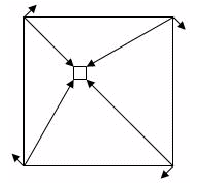
\includegraphics[scale=0.9]{perlinDemonstrationSchema.png}}
		 	\caption{Определение высоты в точке внутри ячейки сетки}
		 	\label{perlinDemonstrationSchema}
	 	\end{figure}
	\indent Поверх уже сгенерированного шума можно наложить ещё один шум, меньшей частоты и более частой сетки, что придаст ландшафту реалистичный вид. Этот способ позволяет легко повторить генерацию, достаточно знать только вектора в каждом угле сетки.
	\paragraph{ Холмовой алгоритм }
	\indent Изначально считается, что все точки находятся на одной высоте, в дальнейшем в произвольных местах задаются холмы различной высоты и диаметра. В результате наложения холмов друг на друга получается ландшафт \cite{hillAlg}.
	\paragraph{ Diamond-square алгоритм }
	Этот алгоритм рекурсивен. Изначально вся карта накрывается одной ячейкой и каждой вершине этой ячейки случайным образом присваивается высота. Далее происходит этап square - в квадрате определяется центральная точка, путем усреднения угловых и добавления случайного отклонения. Далее происходит этап diamond - определяются высоты точек, лежащих в серединах сторон. Для этого используются как точки, лежащие сверху и снизу, так и точки справа и слева, найденные на шаге square. Далее происходит рекурсивное повторение этого алгоритма для каждого квадрата. Заметим, что так как в шаге diamond используются точки, полученные на шаге square, то шаг square проводится для всех текущих квадратов, так же, как и шаг diamond для всех получившихся ромбов. Для простоты применения этого алгоритма необходимо использовать квадратную карту со стороной, равной степени двойки \cite{diamond-square}.
	\\ \indent На рисунке \hyperref[diamondSquareDemonstrationSchema]{\ref{diamondSquareDemonstrationSchema}} визуально представлена одна итерация этого алгоритма.
	\begin{figure}[H]
		 	\center{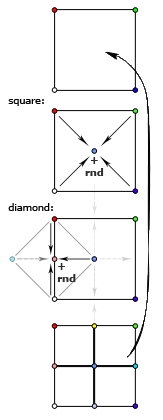
\includegraphics[scale=0.9]{diamondSquareDemonstrationSchema.png}}
		 	\caption{Алгоритм diamond-square}
		 	\label{diamondSquareDemonstrationSchema}
	 	\end{figure}
	\paragraph{Сравнение}
	\indent В таблице \hyperref[noizeCompare]{\ref{noizeCompare}} представлено общее сравнение вышеперечисленных способов генерации карты высот.

	\begin{table}[H]
	\centering
		\caption{Сравнение способов генерации карты высот} \label{noizeCompare}
	\begin{tabularx}{\textwidth}{| Y | Y | Y | Y |}
	\hline
	& Возможность влиять на генерацию & Возможность повторения генерации \\ \hline
	Шум Перлина & + & +  \\ \hline
	Холмовой алгоритм & - & -  \\ \hline
	Diamond-square & + & -  \\ \hline
	\end{tabularx}
	\end{table}
	\paragraph{Вывод}
	\indent Шум Перлина предоставляет более гибкую настройку, позволяя накладывать несколько шумов разной частоты и меняя шаг сетки. Для получения такого же предсказуемого эффекта при генерации другими алгоритмами потребуется дополнительная обработка шумом Перлина, поэтому было принято решение изначально использовать шум Перлина. 
	\subsection{Построение трехмерного изображения на основе карты высот}
	\indent Построение изображения на основе карты высот можно разделить на следующие этапы:
	\begin{enumerate}
		\item разбиение на полигоны;
		\item удаление невидимых граней и поверхностей;
		\item затенение.
	\end{enumerate}
	Рассмотрим каждый этап.
	\subsubsection{Разбиение на полигоны}
	\indent Самым простым многоугольником является треугольник и, как следствие, с первого взгляда было бы логично разбить модель на треугольные полигоны. Но у треугольных полигонов есть несколько недостатков. Так, треугольные полигоны хуже деформируются и могут создавать артефакты, что, при условии совместимости со сторонними редакторами, может привести к нежелательным сложностям. Четырехугольные же полигоны, помимо легкости в деформации, позволяют уменьшить количество вычислений без существенного снижения качества \cite{polygons}.
	\\ \indent Было принято решение использовать четырехугольные полигоны.
	\subsubsection{Удаление невидимых граней и поверхностей}
	\indent Рассмотрим некоторые алгоритмы удаления невидимых граней и поверхностей:
	\begin{enumerate}
		\item алгоритм, использующий Z-буфер;
		\item алгоритм художника;
		\item метод трассировки лучей.
	\end{enumerate}
	Рассмотрим каждый из них.
	\paragraph{ Алгоритм, использующий Z-буфер}
	\indent Алгоритм работает в пространстве изображения. Идея алгоритма крайне проста. Создается буфер, хранящий z-координату каждого пикселя изображения, и заполняется минимальным значением. При обработке очередного пикселя, значение его z-координаты сравнивается с хранящимся в буфере и, если его координата больше хранящейся, то её значение заносится в буфер, а сам пиксель выводится на экран, закрашивая предыдущий \cite{z-buf}.
	\indent Заметим, что размер буфера будет равен размеру пространства изображения. Тем самым, память, требуемая для работы алгоритма, определяется размерами изображения. Основным плюсом данного алгоритма является простота реализации и возможность обрабатывать полигоны объекты в произвольном порядке.
	\paragraph{ Алгоритм художника}
	\indent Идея алгоритма заключается в том, чтобы изображать объекты начиная с самых удаленных от наблюдателя. Для использования алгоритма художника сначала необходимо провести сортировку объектов по глубине и занести их в список приоритетов. В окончательном списке никакие из двух элементов не должны перекрывать друг друга. После этого объекты отображаются, начиная с самого удаленного от наблюдателя \cite{drawerAlg}.
	\indent При использовании данного алгоритма существует сильная зависимость скорости работы от взаимного расположения объектов. Так, при циклическом перекрытии многоугольников используются сложные тесты, для определения ближайщего к наблюдателю. В худшем случае многоугольники необходимо разбивать на несколько новых.
	\paragraph{ Трассировка лучей }
	\indent В этом методе через каждый пиксель картинной плоскости выпускается луч. Из всех граней, с которыми этот луч пересекся, выбирается ближайшая, и точка пересечения отображается.
	\\ \indent С помощью данного метода возможно построения высококачественных изображений, алгоритм легко распараллеливается, вычислительная сложность слабо зависит от сложности сцены. Существенным же минусом является низкая производительность \cite{ray-tracing}.
	\paragraph{Сравнение}
	\indent В таблице \hyperref[paintCompare]{\ref{paintCompare}} представлено сравнение вышеперечисленных алгоритмов.

	\begin{table}[H]
	\centering
		\caption{Сравнение алгоритмов визуализации} \label{paintCompare}
	\begin{tabularx}{\textwidth}{| Y | Y | Y | Y |}
	\hline
	& Маленькая вычислительная сложность & Легкость реализации & Работа с произвольными входными данными \\ \hline
	Алгоритм, использующий Z-буфер & + & + & + \\ \hline
	Алгоритм художника & + & +  & - \\ \hline
	Трассировка лучей & - & -  & + \\ \hline
	\end{tabularx}
	\end{table}
	\paragraph{Вывод}
	\indent Из проведенного сравнения видно, что наиболее оптимальным алгоритмом, в отсутствии требования к фотореалистичному изображению, является алгоритм, использующий Z-буфер.
	\subsubsection{Затенение}
	\indent  В моделях затенения освещенность складывается фоновой, диффузной и зеркальной составляющих \cite{shadowingPart}.
	\\ \indent Фоновая составляющая - некоторая константа освещения, присутствующая в каждой точке, вне зависимости от расположения точки и источника света.
	\\ \indent Дифузная составляющая - это компонента, отвечающая за рассеивание света после попадания на поверхность.
	\\ \indent Зеркальная составляющая отвечает за моделирование отражающих свойств материала. Её добавление позволяет отобразить блики на поверхности.
	\\ \indent На рисунке \hyperref[shadowDemonstration]{\ref{shadowDemonstration}} визуально представлены все компоненты затенения и получившееся изображения.
	\begin{figure}[H]
		 	\center{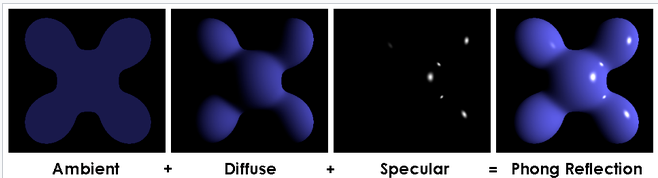
\includegraphics[scale=0.9]{shadowDemonstration.png}}
		 	\caption{Компоненты затенения}
		 	\label{shadowDemonstration}
	 	\end{figure}
	\indent Основные модели затенения:
	\begin{enumerate}
		\item затенение по Ламберту;
		\item затенение по Гуро;
		\item затенение по Фонгу.
	\end{enumerate}
	Рассмотрим каждый из них подробнее.
	\paragraph{Затенение по Ламберту}
	\indent Модель затенения по Ламберту является одной из самых простейших и позволяет описать идеальное диффузное освещение. Если N - вектор нормали в некоторой точке, L - вектор, направленный на источник света, а $I_{ambient}$ - фоновая составляющая, то освещённость по модели Ламберта считается по формуле \hyperref[lambertFormula]{(\ref{lambertFormula})}:
	\begin{equation}\label{lambertFormula}
			 I = I_{ambient} + max(0, dotProduct(N, L))
           \end{equation}
	Затенение по Ламберту предполагает выбор случайной точки на полигоне и экстраполирование цвета этой точки на весь полигон, что создает явный полигональный характер изображения \cite{shadowingLambert}.
	\paragraph{Затенение по Гуро}
	\indent При затенении по Гуро сначала считаются интенсивности света в каждой вершине, а после использкется билинейная интерполяция интенсивностей, что убирает явную дискретность освещения. В этом методе может быть неверно определена зеркальная составляющая, так как происходит усреднение векторов нормалей. В методе гуро учитывается зеркальная составляющая, что отражено в формуле \hyperref[guroFormula]{(\ref{guroFormula})}, использующейся для подсчета интенсивности \cite{shadowingGuro}.
	\begin{equation}\label{guroFormula}
			 I = I_{ambient} + kd * max(0, dotProduct(N, L)) + ks * {max(0, dotProduct(N, \frac{L + V}{|L + V|}))}^{SpecularPower},
           \end{equation}
	где N, L, $I_{ambient}$ тоже, что и в затенении по Ламберту, kd и ks - коэффиценты рассеивания и зеркального освещения соответственно, V - вектор, направленный из точки к наблюдателю, SpecularPower - коэффицент блеска материала.
	\paragraph{Затенение по Фонгу}
	\indent Формула для расчета интенсивности при затенении по Фонгу совпадает с формулой \hyperref[guroFormula]{(\ref{guroFormula})}, но происходит не интерполирование интенсивностей, а интерполирование нормалей, что дает более точный учет зеркальной составляющей. Изображение получается более реалистичным, чем в методе Гуро, но трудоемкость также повышается \cite{shadowingPart}.

	\paragraph{Сравнение}
	\indent В таблице \hyperref[shadowCompare]{\ref{shadowCompare}} представлено сравнение вышеперечисленных моделей затенения.

	\begin{table}[H]
	\centering
		\caption{Сравнение моделей затенения} \label{shadowCompare}
	\begin{tabularx}{\textwidth}{| Y | Y | Y | Y |}
	\hline
	& Маленькая вычислительная сложность & Устранение дискретизации закраски & Учет зеркальной составляющей \\ \hline
	Затенение по Ламберту & + & - & - \\ \hline
	Затенение по Гуро & + & +  & + \\ \hline
	Затенение по Фонгу & - & +  & + \\ \hline
	\end{tabularx}
	\end{table}
	\paragraph{Вывод}
	\indent Из рассмотренных моделей затенения была выбрана модель затенения по Гуро, из-за небольшой вычислительной сложности и учета зеркальной составляющей.

	\subsection{Постановка задачи}
	\indent Разработать программное обеспечение, позволяющее генерировать и отображать ландшафт, представленный в виде карты высот. При генерации использовать шум Перлина. Дать возможность пользователю влиять на генерируемый ландшафт, путем изменения количества узлов сетки и добавления шумов меньшей частоты поверх сгенерированного ландшафта. При отображении использовать алгоритм Z-буфера и затенение по Гуро.
	\subsection{Вывод}
	\indent В данном разделе были рассмотренны и проанализированы существующие алгоритмы решения задачи генерации и отображения ландшафта, уточнены требования к разрабатываемому ПО.
	\newpage
	\section{Конструкторская часть}
	
	\newpage
	\section{Технологическая часть}
	

	\newpage
	\section{Экспериментальная часть}
	
	\subsection{Вывод}

	\newpage
	\begin{center}
		\section*{Заключение}
	\end{center}
	\addcontentsline{toc}{section}{Заключение}
	\newpage
	\addcontentsline{toc}{section}{Список литературы}
	
	\begin{center}
	\begin{thebibliography}{3}
	\bibitem{height-map}
	Карта высот. Wikipedia [Электронный ресурс]. Режим доступа: (дата обращения - 08.12.2020) Свободный. URL: https://en.wikipedia.org/wiki/Heightmap
	\bibitem{vertexAnd}
Генерация трехмерных ландшафтов [Электронный ресурс]. Режим доступа: (дата обращения - 08.12.2020) Свободный. URL: https://www.ixbt.com/video/3dterrains-generation.shtml
	\bibitem{mapPart}
Генерация трехмерных ландшафтов [Электронный ресурс]. Режим доступа: (дата обращения - 08.12.2020) Свободный. URL: https://www.ixbt.com/video/3dterrains-generation.shtml
	\bibitem{perlinNoise}
Шум перлина [Электронный ресурс]. Режим доступа: (дата обращения - 08.12.2020) Свободный. URL: https://medium.com/@yvanscher/playing-with-perlin-noise-generating-realistic-archipelagos-b59f004d8401
	\bibitem{hillAlg}
Холмовой алгоритм [Электронный ресурс]. Режим доступа: (дата обращения - 08.12.2020) Свободный. URL: https://www.ixbt.com/video/3dterrains-generation.shtml
	\bibitem{diamond-square}
Diamond-square algorithm [Электронный ресурс]. Режим доступа: (дата обращения - 08.12.2020) Свободный. URL: http://jmecom.github.io/blog/2015/diamond-square/
	\bibitem{polygins}
Polygon Mesh [Электронный ресурс]. Режим доступа: (дата обращения - 08.12.2020) Свободный. URL: https://en.wikipedia.org/wiki/Polygon\_mesh
	\bibitem{z-buf}
Томский политехнический университет [Электронный ресурс]. Режим доступа: (дата обращения - 08.12.2020) Свободный. URL: http://compgraph.tpu.ru/zbuffer.htm
	\bibitem{drawerAlg}
kursgm.ru [Электронный ресурс]. Режим доступа: (дата обращения - 08.12.2020) Свободный. URL: http://kursgm.ru/grpraktik/grafikomp21.htm
	\bibitem{ray-tracing}
Томский политехнический университе [Электронный ресурс]. Режим доступа: (дата обращения - 08.12.2020) Свободный. URL: http://compgraph.tpu.ru/ray.htm
	\bibitem{shadowingPart}
Bui Tuong Phong, Illumination for computer generated pictures, Communications of ACM 18 (1975), no. 6, 311–317
	\bibitem{shadowingLambert}
Ikeuchi, Katsushi (2014). "Lambertian Reflectance". Encyclopedia of Computer Vision. Springer. pp. 441–443.
	\bibitem{shadowingGuro}
Gouraud, Henri (1971). "Continuous shading of curved surfaces" (PDF). IEEE Transactions on Computers. C-20 (6): 623–629. doi:10.1109/T-C.1971.223313.
	\bibitem{d}
[Электронный ресурс]. Режим доступа: (дата обращения - 08.12.2020) Свободный. URL:

	\bibitem{c-sharp}
	Golang [Электронный ресурс]. Режим доступа: (дата обращения - 20.11.2020) Свободный. URL: https://ru.wikipedia.org/wiki/C\_Sharp
	\bibitem{vs}
	Visual Studio [Электронный ресурс]. Режим доступа: (дата обращения - 20.11.2020) Свободный. URL: https://visualstudio.microsoft.com/ru/

	\end{thebibliography}
	\end{center}
\end{document}